\color{blue}

\section{人机交互}
人机交互研究最初是以机器为中心, 心理学家训练选拔员工以适应机器。后来二战期间机器复杂到难以使人适应, 研究重心才转移到以人为中心……[\cite{} 人机交互研究综述,2017]

人机交互有多种形式, 从最初的发展到现在经历了三代的更替,更替的过程彰显了从“硬交互”到“软交互”的过程。 第一个交互时代是鼠标加键盘的时代……第二个交互时代是触摸交互时代, 使人们的双手从键盘和鼠标中解放出来, 人与机器的交互变得更 加 直 接 和 简 单 ……第三个交互时代是感官交互时代,在这个时代,人机交互已经不需要直接的接触,身体控制、感官交互占据主流……[\cite{}, 新媒体语境下的人机交互叙事初探,2018]。人类与机器间的共生合成体可以说是正在形成……而这种合成体威胁了我们这种感觉的稳定性。 人类创造了电脑,接着电脑又创造了新型的人,这也许正在悄然发生。[\cite{}马克·波斯特.信息方式[M].范静哗.译,北京:商务印书馆,2000:11 ]

\section{“强”交互}

机器和设备对于“人的影响”日益明显,甚至正在 “创造新型的人”,这和其本身的存在形式的演变不无关系。在现有的“人机交互”的基础上,我们尝试提出“强交互”的概念,并进一步探究“设备”对人的影响。
2.1、刺激强度
	设备对人刺激强度的不断增加是重要特点。
2.2、软件的“沉浸式设计”
	各类产品的“沉浸式设计”是加强人机交互强度的直接因素,这是一个涉及到心理、设计、游戏等领域的概念。
2.3、相互反馈
人机“强交互”语境下,存在一个人与机器相互反馈,影响双方行为的过程,并形成相对稳定的交互关系,使得用户个人与其设备构筑成为一个共生的“强交互环境”。

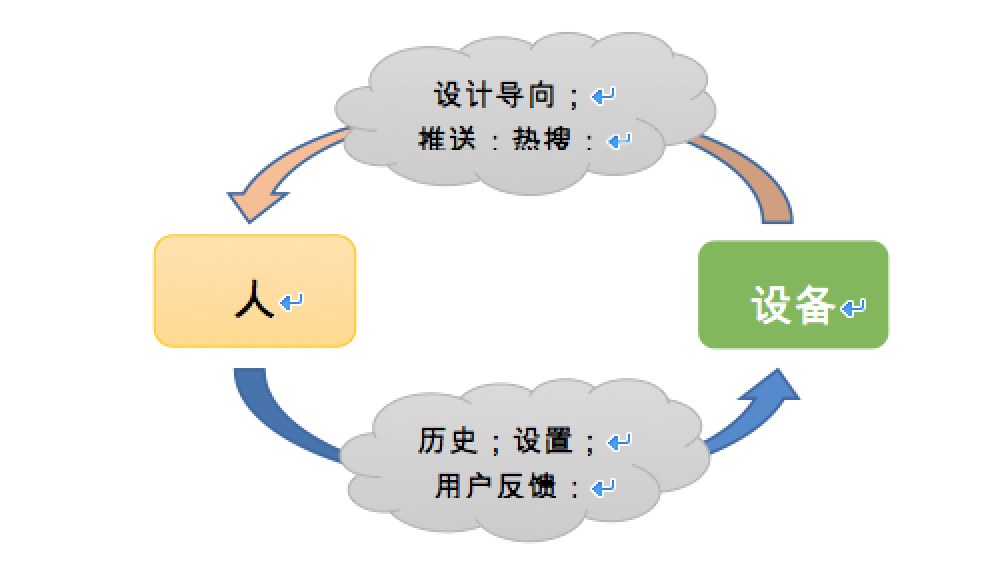
\includegraphics[scale=0.6]{人机交互}

如上图所示,软硬件设计本身就具有明显的导向性,例如抖音等小视频软件的诱导性,包括吸引用户发布视频和游客“沉浸”于浏览视频,微博等公众社交媒体“热搜”等设置有明显的舆论导向甚至价值导向作用;而用户的个人设置,浏览记录等信息使得媒体“更好地”针对性推送内容,使用户与设备的联系进一步加强,大数据背景下的用户反馈又是促使媒体优化设计的重要影响因素,使得“人机交互”成为一个持续的双向强化过程,并在这个过程中打造出一个针对用户个体的适宜、偏好和易沉浸的“强交互环境”。
\section{特征}

现象:设备使用频率和时长的增加
	在“人机强交互环境”中,人们对设备的使用频率在增加(时不时看手机),使用的持续时间变长(一看就是好几十分钟甚至几个小时),使用时的“浸入程度”也在加深(走路都要看,掉下水道里去!)。
		这中现象对人们的生活带来……的直接影响,也在悄然改变我们的思维和认知习惯……balabala……

\section{影响}
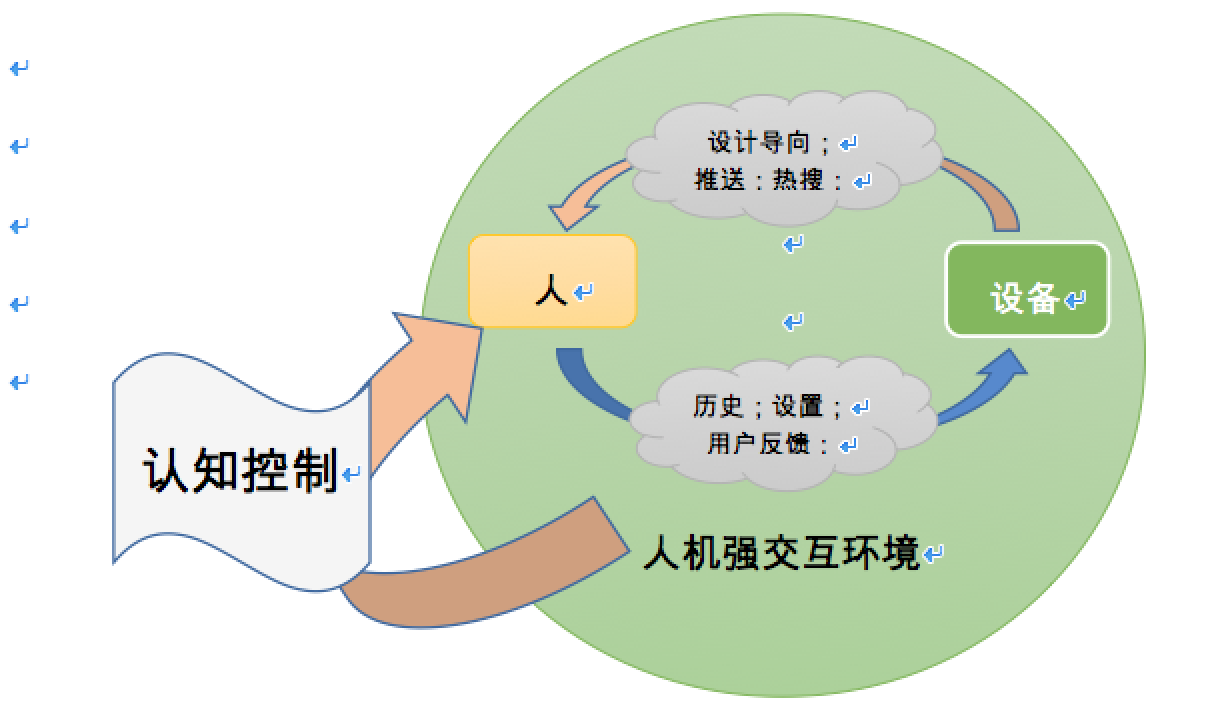
\includegraphics[scale=0.6]{人机强交互-认知控制}
